\errorcontextlines=5

%%%

\documentclass[
%handout,
]{beamer}

\usepackage{ifluatex}
\ifluatex\else\errmessage{This document requires LuaLaTeX}\fi

\usepackage{etex,etoolbox}
\usepackage{fontspec}
\usepackage[ngerman]{babel}
\usepackage{csquotes}
\usepackage{array}
\usepackage{wrapfig}
\usepackage{booktabs}
\usepackage{ccicons}
\usepackage{calc}

\usepackage{tikz}
\usetikzlibrary{arrows,intersections,calc,through,%
  external,positioning,automata,datavisualization,%
  datavisualization.formats.functions}

\usepackage{luacode}
\usepackage{pgfplots}
\usepackage{manfnt}

%%% title and such

\title{Wissenschaftliches Arbeiten mit \LaTeX}
\author{\texorpdfstring{Felix Hilsky\\basierend auf einem Kurs von\\Daniel Borchmann,\\Tom Hanika und \\Max Marx}{Felix Hilsky basierend auf einem Kurs von Daniel Borchmann, Tom Hanika und Max Marx}}
\titlegraphic{\ccLogo \ccAttribution \ccShareAlike}

%%% theme

\usepackage{tikz}
\usetikzlibrary{shapes.multipart}
\usetheme{CambridgeUS}
\setbeamertemplate{blocks}[rounded][shadow=false]
\setbeamertemplate{items}{\raisebox{0.3ex}{%
    \tikz[scale=0.13] \draw[fill] (0,0) -- (0,1) -- (0.9,0.5) -- cycle;}}
\usetikzlibrary{arrows}
\tikzset{>={stealth'[sep]}}
\setbeamertemplate{navigation symbols}{}
\setbeamertemplate{footline}{}
\setlength{\abovedisplayskip}{0pt}
\setbeamerfont{title}{series=\bfseries}
\defbeamertemplate{block alerted begin}{bends}{%
  \begin{columns}
    \begin{column}{0.05\linewidth}
      \dbend
    \end{column}
    \begin{column}{0.95\linewidth}
      \vskip.75ex\usebeamercolor[fg]{block title
        alerted}\insertblocktitle{}
      \vskip.1em
      \usebeamercolor[fg]{normal text}
}
\defbeamertemplate{block alerted end}{bends}{%
    \end{column}
  \end{columns}
}
%%%

\mode<handout>{
  \usepackage{pgfpages}
  \pgfpagesuselayout{2 on 1}[a4paper,border shrink=5mm]
}

%%% lecture organization

\usepackage{xparse}
\DeclareDocumentCommand \Lecture { m m }{%
  \lecture{#1}{#2}
  \part{#1}
  \include{#2}
}

\AtBeginSection{
  \setbeamertemplate{blocks}[rounded][shadow=true]
  \begin{frame}[plain]
    \begin{block}{}
      \begin{center}
        \textcolor{darkred}{\textbf{\Large \strut\smash{\insertpart}}}\\[1ex]
        \textcolor{blue!70!black}{\strut\smash{\insertsection}}
      \end{center}
    \end{block}
  \end{frame}
  \setbeamertemplate{blocks}[rounded][shadow=false]
  \setbeamertemplate{block alerted begin}[bends]
  \setbeamertemplate{block alerted end}[bends]
}

%%% misc

\newcommand{\GNULinux}{GNU\lower-0.25ex\hbox{/}Linux}
\newcommand{\TikZ}{Ti\emph{k}Z}

\usepackage{listings}

\lstset{language=[LaTeX]TeX, basicstyle=\ttfamily,
  keywordstyle={\color{blue}\bfseries}, frame=tb, extendedchars=true, literate=%
  {ä}{{\"a}}1 {ö}{{\"o}}1, escapeinside={(*@}{@*)}, mathescape=true,
  basewidth=0.5em, keywordstyle={\color{blue}},
  morekeywords={[0]includegraphics,rotatebox,scalebox,resizebox,providecommand,
    subsection,subsubsection,paragraph,subparagraph,part,chapter,tableofcontents,
    mathring,text,mathbb,printindex,addbibresource,printbibliography,subtitle,
    institute,titlegraphic,subject,keywords,draw,path,color,textcolor,toprule,
    midrule,bottomrule,maketitle,setlength,enquote,listoffigures,listoftables,
    theoremstyle,theoremheaderfont,theorembodyfont,newblock,parencite,footcite,
    autocite,bibitem,middle,tikzset,usetikzlibrary,coordinate,node,foreach,
    datavisualization,varepsilon,autocite,bibitem,DeclareRobustCommand,
    DeclareDocumentCommand,IfBooleanTF,bye,frametitle,setbeamertemplate,pause,
    onslide,uncover,visible,invisible,only,alt,temporal,alert,AtBeginSection,
    usetheme,setbeamerfont,tikz,includeonlyframes,mode,pgfpagesuselayout,RequirePackage,
  },
}

\AtBeginDocument{\frame[plain]{\maketitle}}

%%% end of preamble
\subtitle{Präsentationen}
\date{2017-05-29}

\begin{document}

\begin{frame}[label=ziel]
  \frametitle{Ziel dieses Abschnittes}

  \onslide<+->
  \begin{itemize}
  \item Erstellung von Präsentationen mit \LaTeX\texttt{-beamer}
  % \item \enquote{Vieles, was Powerpoint kann} (nur schöner)
  % \item Fallstricke und Tipps zur Erstellung von Präsentationen mit \LaTeX
  \end{itemize}

  \onslide<+->

  \bigskip

  Mehr Details in der Dokumentation von \texttt{beamer}:\\
  \vspace*{\baselineskip}
  \qquad\texttt{\$ texdoc beamer} bzw.\ \url{ctan.org/pkg/beamer}\\
  \vspace*{\baselineskip}
  Die Dokumentation ist sehr verständlich und oft unterhaltsam!
  % auf der Kommandozeile (ohne \texttt{\$}; das ist der Prompt)

\end{frame}

\section{\LaTeX\texttt{-beamer}}

% \begin{frame}
%   \frametitle{Was ist und was soll \LaTeX-\texttt{beamer}?}

%   \onslide<1->

%   \begin{wrapfigure}{r}{3cm}
%     \onslide<3->{%
%       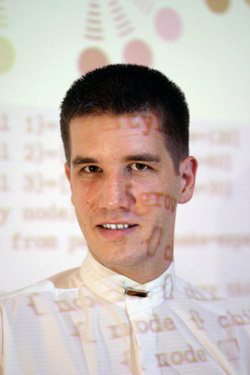
\includegraphics[width=\linewidth,keepaspectratio]{pics/till-tantau}\\[-0.5\baselineskip]
%       \scalebox{0.3}{\url{http://www.tcs.uni-luebeck.de/mitarbeiter/tantau/}}}
%   \end{wrapfigure}
%   ~
%   \begin{itemize}
%   \item<1-> \LaTeX-\texttt{beamer} ist eine Dokumentenklasse für das Erstellen von
%     Präsentationen mit \LaTeX
%   \item<+-> Entwickelt von Till Tantau, weiter betreut von Joseph Wright and Vedran
%     Miletić
%   \item<+-> Verbindet Präsentationen mit der typographischen Qualität von \TeX
%   \item<+-> Weit verbreitet in der akademischen Welt (und darüber hinaus?)
%   % \item<6-> Präsentationen ähnlich zu anderen Systemen (meist aber etwas
%   %   \enquote{statischer})
%   \item<+-> Einfach zu bedienen (wenn man \LaTeX kennt)
%   \end{itemize}

% \end{frame}

\section{Grundaufbau einer Präsentation mit \LaTeX\texttt{-beamer}}

% We define a new frame environment here, so we can use `\end{frame}' in
% listings on the slides (otherwise beamer will look for `\end{frame}' as the
% end of the current frame, and will get confused by the `\end{frame}' in the
% code listing).

\newenvironment{slide}
  {\begin{frame}[fragile,environment=slide]}
  {\end{frame}}

% Hm, vielleicht mal die Dokumentenklasse erwähnen … ?

\begin{slide}
  \frametitle{Frames}

  \onslide<+->
  Die Dokumentenklasse ist \lstinline|beamer|.
\begin{lstlisting}
\documentclass{beamer}
\end{lstlisting}
  \onslide<+->

  Einzelne Folien werden mit \lstinline!\begin{frame}! \dots \lstinline! \end{frame}!
  erzeugt:
\begin{lstlisting}
\begin{frame}
  \frametitle{Frames}
  $\dots$
\end{frame}
\end{lstlisting}

  % \onslide<+->

  % Hinter \lstinline!\begin{frame}! können noch Optionen in \lstinline![...]! angegeben
  %   werden:
  % \begin{itemize}
  %   \item \lstinline!label=$\textit{name}$!, um einzelnen Folien Label zu geben. % hilft ja nicht, wenn man die Foliennummer als Zuhörer sehe...
  % \item \lstinline{fragile}, falls die Folie \lstinline{verbatim}-Text oder Listings (\enquote{Quellcode})
  %   enthält
  % \item \lstinline{plain}, falls die Folie keine Kopf- und Fußzeile haben soll
  % \item \lstinline{shrink}, \lstinline{squeeze}, \lstinline{b}, \lstinline{c},
    % \lstinline{t}, 
    % \dots
  % \end{itemize}
  Innerhalb von \lstinline|frames| schreibt man gewohntes \LaTeX.

\end{slide}

\begin{slide}
  \frametitle{Spalten}
  \begin{columns}
    \begin{column}{0.4\textwidth}
      Oft ist es praktisch die Folie in (zwei) Spalten zu teilen.

      Zum Beispiel um ein Bild neben Text zu platzieren.
    \end{column}
    \begin{column}{0.6\textwidth}
\begin{lstlisting}
\begin{columns}
 \begin{column}{0.5\textwidth}
  Text
 \end{column}
 \begin{column}{0.5\textwidth}
   \includegraphics[
     width=0.4\textwidth]{Bild}
 \end{column}
\end{columns}
\end{lstlisting}
    \end{column}
  \end{columns}
\end{slide}

\begin{slide}
  \frametitle{Blöcke}

  \onslide<+->

  Einträge auf einer Folie können in \emph{Blöcken} gruppiert werden:

\begin{lstlisting}
\begin{block}{Titel}
  Text Text Text
\end{block}
\end{lstlisting}

  \onslide<+->

  \begin{block}{Titel}
    Text Text Text
  \end{block}

  \onslide<+->

  Vordefinierte Blöcke: \texttt{Satz}, \texttt{Beweis}, \texttt{Beispiel}, \dots (Ja, deutsche Namen!)

  % Je nach Theme können die Blöcke auch Schatten haben:

  \setbeamertemplate{blocks}[rounded][shadow=true]
  \begin{Satz}<+->[Euklid]
    Es gibt unendlich viele Primzahlen.
  \end{Satz}
  \setbeamertemplate{blocks}[rounded][shadow=false]

  \onslide<+->
  Blöcke sind in vielen Themes hervorgehoben.
\end{slide}

\section{Overlays}

\begin{slide}
  \frametitle{Overlay-Kommandos}

  \onslide<+->

  Beamer stellt verschiedene Möglichkeiten bereit, Dinge nach und nach einzublenden. Diese heißen \textit{overlays}.
  % sagen:
   % zu erzeugen, welche
  % dann als aufeinander folgenden Seiten im erzeugten Dokument dargestellt werden:

  \onslide<+->

  \begin{itemize}
  \item \lstinline{\pause} (simpel, reicht meistens)
  \item \lstinline{\onslide}
  \item \lstinline{\uncover}
  \item \lstinline{\visible}, \lstinline{\invisible}
  \item \lstinline{\only}
  \item \lstinline{\alt}, \lstinline{\temporal}, \lstinline{onlyenv},
    \lstinline{overprint}, \lstinline{altenv}, \lstinline{overlayarea}, \dots
  \end{itemize}

  \onslide<+->

  Mit Hilfe von \lstinline{\pause} können einzelne Abschnitte nacheinander aufgedeckt
  werden.

  \onslide<+->

  Alle anderen Anweisungen werden durch \emph{Overlay-Spezifikationen} gesteuert.

\end{slide}

\begin{slide}
  \frametitle{Overlay-Spezifikationen}
  Overlay-Spezifikationen geben an, auf welchen Folien etwas (nicht) angezeigt wird. Sie werden in spitze Klammern gesetzt.
  \onslide<+->

  \begin{Beispiele}
\begin{lstlisting}
\onslide<2-4>{Ich bin ein Text}
\end{lstlisting}
    erscheint auf Folien 2 bis 4 (inklusive); Text nimmt aber Platz ein, auch wenn er
    nicht gezeigt wird.
    \onslide<+->
\begin{lstlisting}
\onslide<2->{Ich bin noch ein Text}
\end{lstlisting}
    erscheint auf Folie 2 und bleibt bis zum Ende.
    % Ende kann weggelassen werden
    \onslide<+->
\begin{lstlisting}
\onslide<-4>{Text Text Text}
\end{lstlisting}
    erscheint von Anfang an, verschwindet dann aber auf Folie 5
    % Anfang kann weggelassen werden
    \onslide<+->
\begin{lstlisting}
\onslide<2->  % fehlendes Argument bedeutet "alles weitere"
Kreativität darf man hier nicht erwarten \dots
\end{lstlisting}
    Alles im aktuellen Frame wird erst auf Folie 2 und folgend angezeigt.
    % Insbesondere ist das Argument in {} ein optionales Argument!
  \end{Beispiele}

\end{slide}

\begin{slide}
  \frametitle{Overlay-Spezifikationen}

  \onslide<+->

  \begin{block}{\textcolor{red}{Problem}}
    Die explizite Angabe von Folien-Nummern ist unhandlich.
  \end{block}

  \onslide<+->

  Aber es geht auch ohne!

  \onslide<+->

  \begin{Beispiele}
\begin{lstlisting}
\onslide<+->
\end{lstlisting}
    Alles, was dieser Anweisung folgt, wird auf der \emph{nächsten} Folie aufgedeckt.
    \onslide<+->
\begin{lstlisting}
\onslide<+->{Teeeeeeeext}
\end{lstlisting}
    Der Text wird auf der folgenden Folie angezeigt.
    % \onslide<+->
% \begin{lstlisting}
% \onslide<.->{Texxxxxxxxxt}
% \end{lstlisting}
%     Der Text wird auf der \emph{aktuellen} Folie mit angezeigt. (sinnvoll mit
%     \lstinline{\alert} statt \lstinline{\onslide})
  \end{Beispiele}

\end{slide}

\begin{slide}
  \frametitle{Weitere Anweisungen mit Overlay-Spezifikationen}

  \onslide<+->

  \begin{Beispiele}
\begin{lstlisting}
\alert<2>{ACHTUNG!}
\end{lstlisting}
    Zeigt \alert<.>{ACHTUNG!} auf Folie 2 hervorgehoben an.
    \onslide<+->
\begin{lstlisting}
\item<+-> Noch ein Text ohne Sinn
\end{lstlisting}
    Zeigt den entsprechenden Punkt auf der nächsten Folie an
    \begin{overprint}[\linewidth] % linewidth ist auch default
      \onslide<+| handout:0>
\begin{lstlisting}
\begin{itemize}
\item<+-> Foo
\item<+-> Bar
\item<+-> Baz
\end{itemize}
\end{lstlisting}
      \onslide<+-| handout:1>
\begin{lstlisting}
\begin{itemize}[<+->] % Standardwert für alle items
\item Foo
\item Bar
\item Baz
\end{itemize}
\end{lstlisting}
    \end{overprint}
  \end{Beispiele}

\end{slide}

\section{Struktur}

\begin{slide}
  \frametitle{Titelfolie}

  Eine Titelfolie kann einfach erstellt werden:
\begin{lstlisting}
\frame{\titlepage}
\frame[plain]{\titlepage}
\frame[plain]{\maketitle}
\end{lstlisting}

  \onslide<+->

  Die Kommandos \lstinline{\author}, \lstinline{\title}, \lstinline{\subtitle},
  \lstinline{\date} funktionieren wie gewohnt.
  % subtitle von KoMa-Klasse

  \onslide<+->

  Darüber hinaus gibt es noch \lstinline{\institute}, \lstinline{\titlegraphic},
  \lstinline{\subject}, \lstinline{\keywords}.

\end{slide}

\begin{slide}
  \frametitle{Abschnitte}

  \onslide<+->

  Abschnitte werden wie \LaTeX\ üblich mit \lstinline{\section}, \dots\ angelegt

\begin{lstlisting}
\section{Overlays}
\end{lstlisting}

  \onslide<+->

  Je nach Theme wird dies dann in den Kopf- oder Fußzeilen der Folien angezeigt. Es wird nicht automatisch eine Überschrift erzeugt.
\end{slide}

\begin{slide}
  \frametitle{Inhaltsverzeichnis}

  \onslide<1->

  Einfach wie üblich mit
\begin{lstlisting}
\tableofcontents
\end{lstlisting}

  \onslide<2->{\tableofcontents}

\end{slide}

\begin{slide}
  \frametitle{Inhaltsverzeichnis}

  \onslide<1->

  Optionen sind auch möglich
\begin{lstlisting}
\tableofcontents[currentsection]
\end{lstlisting}

  \onslide<2->{\tableofcontents[currentsection]}

\end{slide}

% \begin{slide}
%   \frametitle{Inhaltsverzeichnis}

%   \onslide<+->

% \begin{lstlisting}
% \AtBeginSection{%
%   \tableofcontents[currentsection]
% }
% \end{lstlisting}
%   zeigt bei jedem neuen Abschnitt an, wo man sich gerade in der Präsentation befindet.

% \end{slide}

\section{Aussehen}

\begin{slide}
  \frametitle{Teile einer Folie}

  \onslide<+->

  Eine Folie hat in \texttt{beamer} folgende Bestandteile
  \begin{itemize}
  \item Kopf- und Fußzeile
  \item Linke und rechte Sidebar
  \item Navigationsleiste
  \item Navigationssymbole
  \item Logo
  \item Folientitel
  \item Hintergrund
  \item Inhalt
  \end{itemize}

  \onslide<+->

  Alle diese Komponenten lassen sich mit Hilfe von \textit{Templates} anpassen. (siehe
  Dokumentation)
% sie ist gut und teilweise unterhaltsam!
  \onslide<+->
  \begin{Beispiel}
\begin{lstlisting}
\setbeamertemplate{navigation symbols}{}
\end{lstlisting}
    deaktiviert die Navigationssymbole in der Präsentation.
  \end{Beispiel}

\end{slide}

\begin{frame}[fragile]
  \frametitle{Farben und Aussehen einstellen}

  \onslide<+->

  \LaTeX-\texttt{beamer} bietet viele Möglichkeiten, das Aussehen anzupassen.  Hier nur
  beispielhaft die Einstellungen für diesen Vortrag: \onslide<+->
\begin{lstlisting}
\usetheme{CambridgeUS}
\setbeamertemplate{blocks}[rounded][shadow=false]
\setbeamertemplate{items}{\raisebox{0.3ex}{%
 \tikz[scale=0.13]%
  \draw[fill] (0,0) -- (0,1) -- (0.9,0.5) -- cycle;}}
\setbeamertemplate{navigation symbols}{}
\setbeamertemplate{footline}{}
\setbeamerfont{title}{series=\bfseries}
\end{lstlisting}
  \onslide<+->

  Viel mehr in der Dokumentation!

\end{frame}

\section{Schnelleres Übersetzen}
\begin{slide}
  \frametitle{Schnelleres Übersetzen}

  \onslide<+->

  \begin{block}{\textcolor{red}{Problem}}
    Mit steigender Zahl von Folien wird die Übersetzung merklich langsamer.
  \end{block}

  \onslide<+->

  \begin{block}{\textcolor{green!50!black}{Lösung}}
    Nur die Folien übersetzen, die aktuell benötigt werden:
\begin{lstlisting}
% in der Präambel
\includeonlyframes{current}
% im Dokument
\begin{frame}[label=current]
  ...
\end{frame}
\end{lstlisting}
  \end{block}

\end{slide}

% \begin{slide}
%   \frametitle{Handouts}

%   \onslide<+->

%   \begin{block}{\enquote{\textcolor{red}{Problem}}}
%     Handouts erstellen.
%   \end{block}

%   \onslide<+->

%   Mit
% \begin{lstlisting}
% \documentclass[handout]{beamer}
% \mode<handout>{%
%   \usepackage{pgfpages}
%   \pgfpagesuselayout{2 on 1}[a4paper,border shrink=5mm]
% }
% \end{lstlisting}

  % \onslide<+->

  % Es sind dann eventuell kleine Anpassungen im Dokument nötig.

% \end{slide}

\end{document}

%%% Local Variables:
%%% mode: latex
%%% TeX-master: t
%%% TeX-engine: luatex
%%% ispell-local-dictionary: "de_DE"
%%% End:

%  LocalWords:  Navigationssymbole Slides Slide Frame
